\chapter{Model and methods}
\label{chap:modmet}
To test the thesis hypothesis, a formulation of the Weather Research and Forecasting (WRF) Model called the Advanced Research WRF (ARW) has been used. The model is described in the first part of this chapter. Then follows a description of the model setup and the different physics schemes that were chosen for this study, before a summary of the different runs that were performed. Ending the chapter are two short sections on the input data and processing of the model output.

%---------------------
\section{Description of the WRF-ARW Modeling System}
\label{sec:modeldes}
%---------------------
The version of the WRF-ARW modeling system used is 3.6.1, which was released in April 2014. The model is primarily developed at the National Centre for Atmospheric Research (NCAR) in Boulder, Colorado. The ARW model is the first fully compressible conservative form nonhydrostatic model designed for both research and operational numerical weather prediction (NWP) applications~\citep{Skamarock2008}. 

As can be seen from figure~\ref{fig:wrfflowchart} the WRF-ARW Modeling System consists of four major programs~\citep{Wang2015}:
\begin{itemize}
\item The WRF Preprocessing System (WPS)
\item WRF-Data Assimilation (WRF-DA)
\item ARW solver
\item Post-processing \& Visualization tools
\end{itemize}

\begin{figure}[ht]
\centering
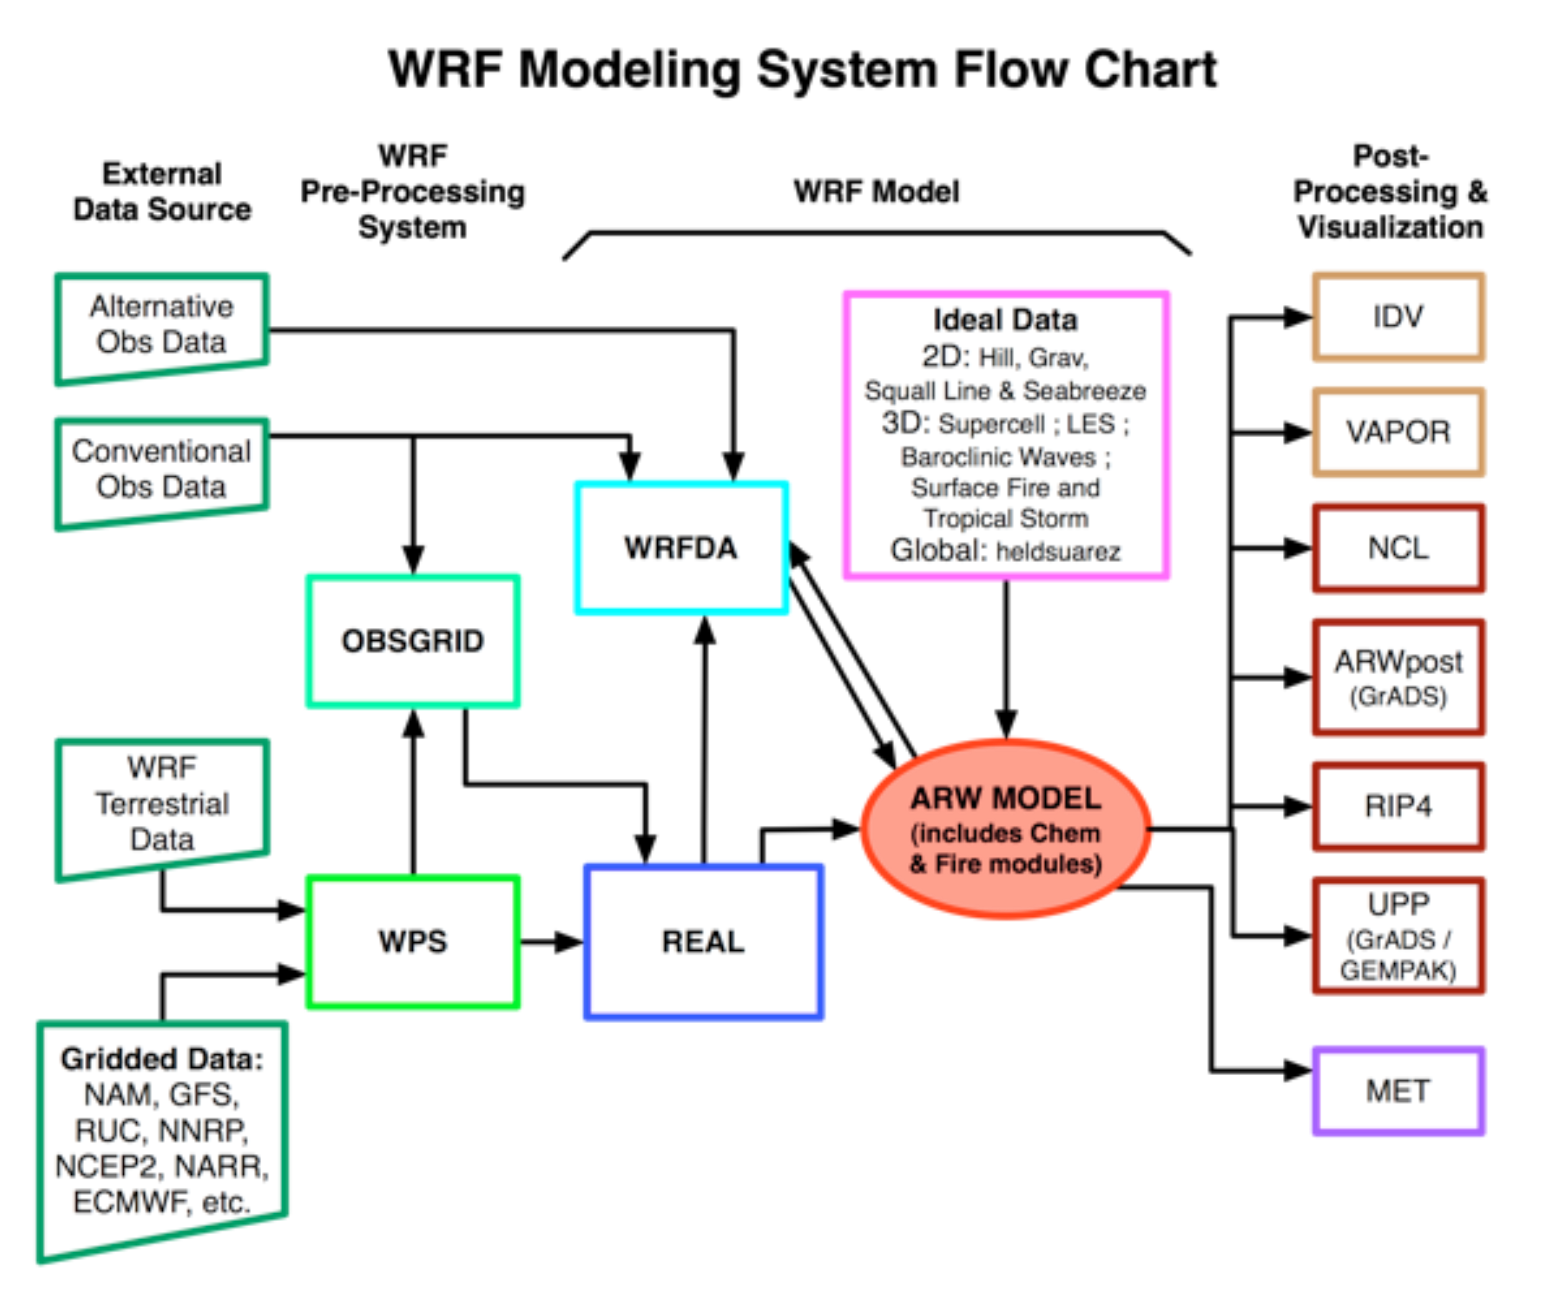
\includegraphics[width=0.9\textwidth]{model_methods/wrfflowchart}
\caption{Flowchart for the WRF ARW Modeling System Version 3. From~\citet{Wang2015}.}
\label{fig:wrfflowchart}
\end{figure}

WPS is used primarily for real data simulations~\citep{Wang2015}, like the study presented in this thesis. A real-data simulation means that it has been initialized by observations and reanalysis, not artificial data. WPS' functions include defining simulation domains, interpolating terrestrial data and degribbing and interpolating meteorological data from another model to this simulation domain~\citep{Wang2015}. WRF-DA is optional and can be used to ingest observations into the interpolated analyses created by WPS~\citep{Wang2015}, but was not used in this study. The ARW solver is the key component of the modeling system, which is composed of several initialization programs for idealized, and real-data simulations, and the numerical integration program~\citep{Wang2015}.% Fully compressible nonhydrostatic equations with hydrostatic options, regional and global applications, complete coriolis and curvature terms and that vertical grid-spacing can vary with height are among the WRF models key features according to~\citet{Wang2015}.

The continuous equations solved in the ARW model are the Euler equations cast in a flux form where the vertical coordinate, $\eta$, is defined by a normalized hydrostatic pressure,
\begin{equation}
\eta = (p_h - p_{ht})/\mu 
\end{equation}
where $\mu = (p_{hs} - p_{ht})$~\citep{Skamarock2008}. $p_h$ is the hydrostatic component of the pressure and $p_{hs}$ and $p_{ht}$ are the values of the hydrostatic pressure in a dry atmosphere at the surface and top boundaries respectively~\citep{Skamarock2008}.

The vertical coordinate is the traditional $\sigma$ coordinate used in many hydrostatic atmospheric models, but is denoted by $\eta$ in ARW, and is shown in figure~\ref{fig:sigma}.

\begin{figure}[ht]
\centering
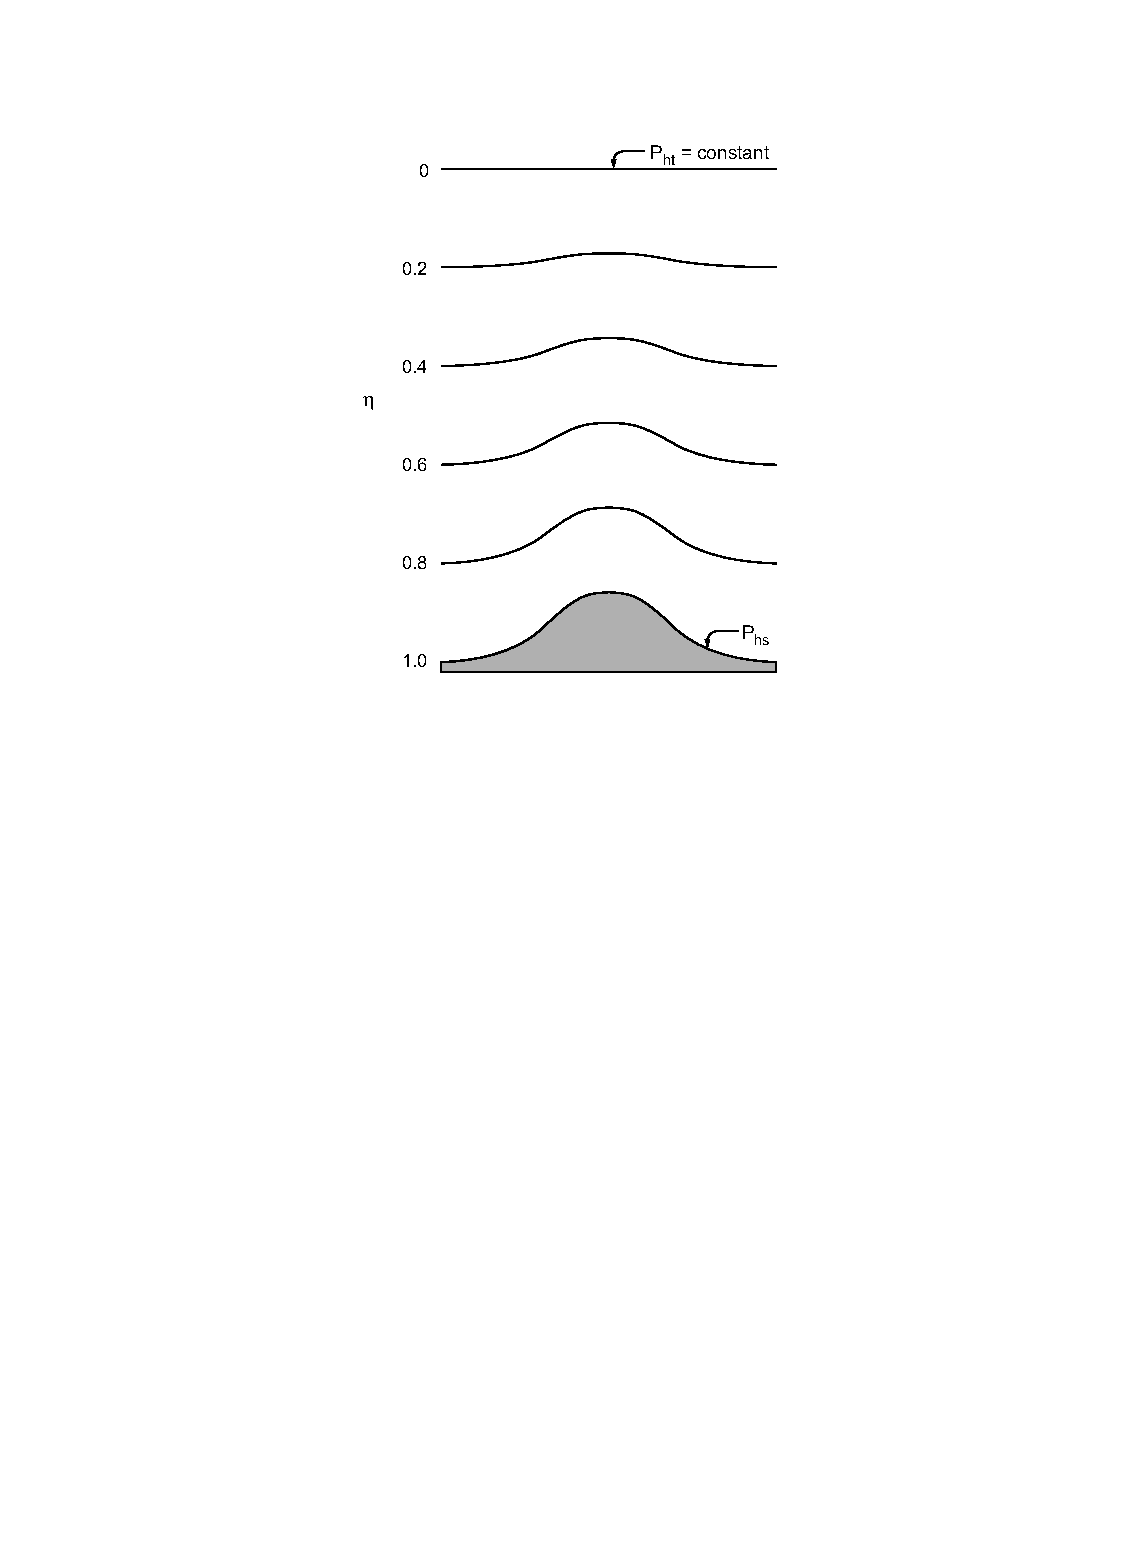
\includegraphics[scale=0.9]{model_methods/sigma.pdf}
\caption{This figure is shown as presented in~\citet{Skamarock2008}, and is a schematic of the $\eta$ coordinate. $P_{hs}$ and $P_{ht}$ represent the hydrostatic pressure at the surface and top respectively.}
\label{fig:sigma}
\end{figure}

$\eta$ decreases monotonically from a value of 1 at the surface, where the coordinate follows the terrain and $P_h = P_{hs}$, to a value of 0 at the top level, which is then a pressure surface, where $P_h = P_{ht}$. Levels with constant $\eta$ are commonly referred to as $\eta$-levels (or Eta-levels). $\mu(x,y)$ is the mass of dry air per unit area within the column in the model domain at $(x,y)$. The $\eta$-levels are where the vertical wind speed is calculated, whereas the thermodynamic variables ($\theta$) are calculated between the $\eta$-levels, on so-called mass levels.

%--------- Stuff on staggered grid.
With the vertical coordinate $\eta$, and the mass of an air column, $\mu(x,y)$, in the model grid the Euler equations can be written with  variables on flux form:
\begin{eqnarray*}
\textbf{V} = \mu \textbf{v} = (U,V,W),\textit{    }\Omega = \mu \dot{\eta},\textit{    }\Theta = \mu \theta
\end{eqnarray*}
Now \textbf{v} is the velocity vector in three dimensions, $\omega = \dot{\eta}$ denotes the vertical velocity and $\phi$ is the geopotential, and the set of prognostic equations that needs to be solved numerically is this:
\begin{eqnarray}
\partial_t U + (\nabla \cdot \textbf{V}_u) - \partial_x (p\phi_{\eta}) + \partial_{\eta}(p\phi_x) &=& F_U\\ \label{eqn:euler1}
\partial_t V + (\nabla \cdot \textbf{V}_v) - \partial_y (p\phi_{\eta}) + \partial_{\eta}(p\phi_y) &=& F_V\\
\partial_t W + (\nabla \cdot \textbf{V}_w) + g(\partial_{\eta}p-\mu)&=&F_W\\
\partial_t \Theta + (\nabla \cdot \textbf{V}\theta) &=& F_{\Theta}\\ \label{eqn:euler2}
\partial_t \mu + (\nabla \cdot \textbf{V}) &=& 0\\
\partial_t \phi + \mu^{-1}[(\textbf{V} \cdot \nabla \phi - gW) &=& 0\\
\partial_t Q_m + (\nabla \cdot \textbf{V}Q_m) &=& F_{Q_m} \label{eqn:euler3}
\end{eqnarray}
To close the system they use the diagnostic equation for inverse density, $\alpha_d$,
\begin{equation}
\partial_{\eta} \phi = -\alpha_d \mu
\end{equation}
and the moist equation of state
\begin{equation}
p = p_0\left(R_d\theta\frac{1+R_d/R_v)q_v}{p_0\alpha_d}\right)^{\gamma}
\end{equation}
where $\gamma = c_v/c_p = 1.4$ is the ratio of the heat capacity for dry air at constant volume, to that of constant pressure, $R_d$ and $R_v$ are the gas constants for dry and moist air respectively, $q_v$ is the mixing ratio of water vapor and $p_0$ is the reference pressure (10$^3$hPa). The right-hand-side terms in equations~\ref{eqn:euler1}-\ref{eqn:euler2} and~\ref{eqn:euler3} represent forcing terms which arise from model physics, turbulent mixing, spherical projections, the earth's rotation, and moist physics~\citep{Skamarock2008a}.

To solve these equations the WRF-ARW modeling system uses the spatial discretization known as a staggered C grid~\citep{Skamarock2008a}. Figure~\ref{fig:stagger} shows the schematic of the grid and how the velocities, $u$ and $v$, are calculated at the edges of each grid box both in the horizontal and in the vertical, half a grid box length away from the thermodynamic variable, which is calculated in the middle of each grid box, at the mass point. The advection in and out of the grid box is calculated from $u$ and $v$. This staggering allows for discretization of the pressure gradient and divergence terms across a single grid interval, without any averaging, which gives a highly accurate second order difference.

\begin{figure}[ht]
\centering
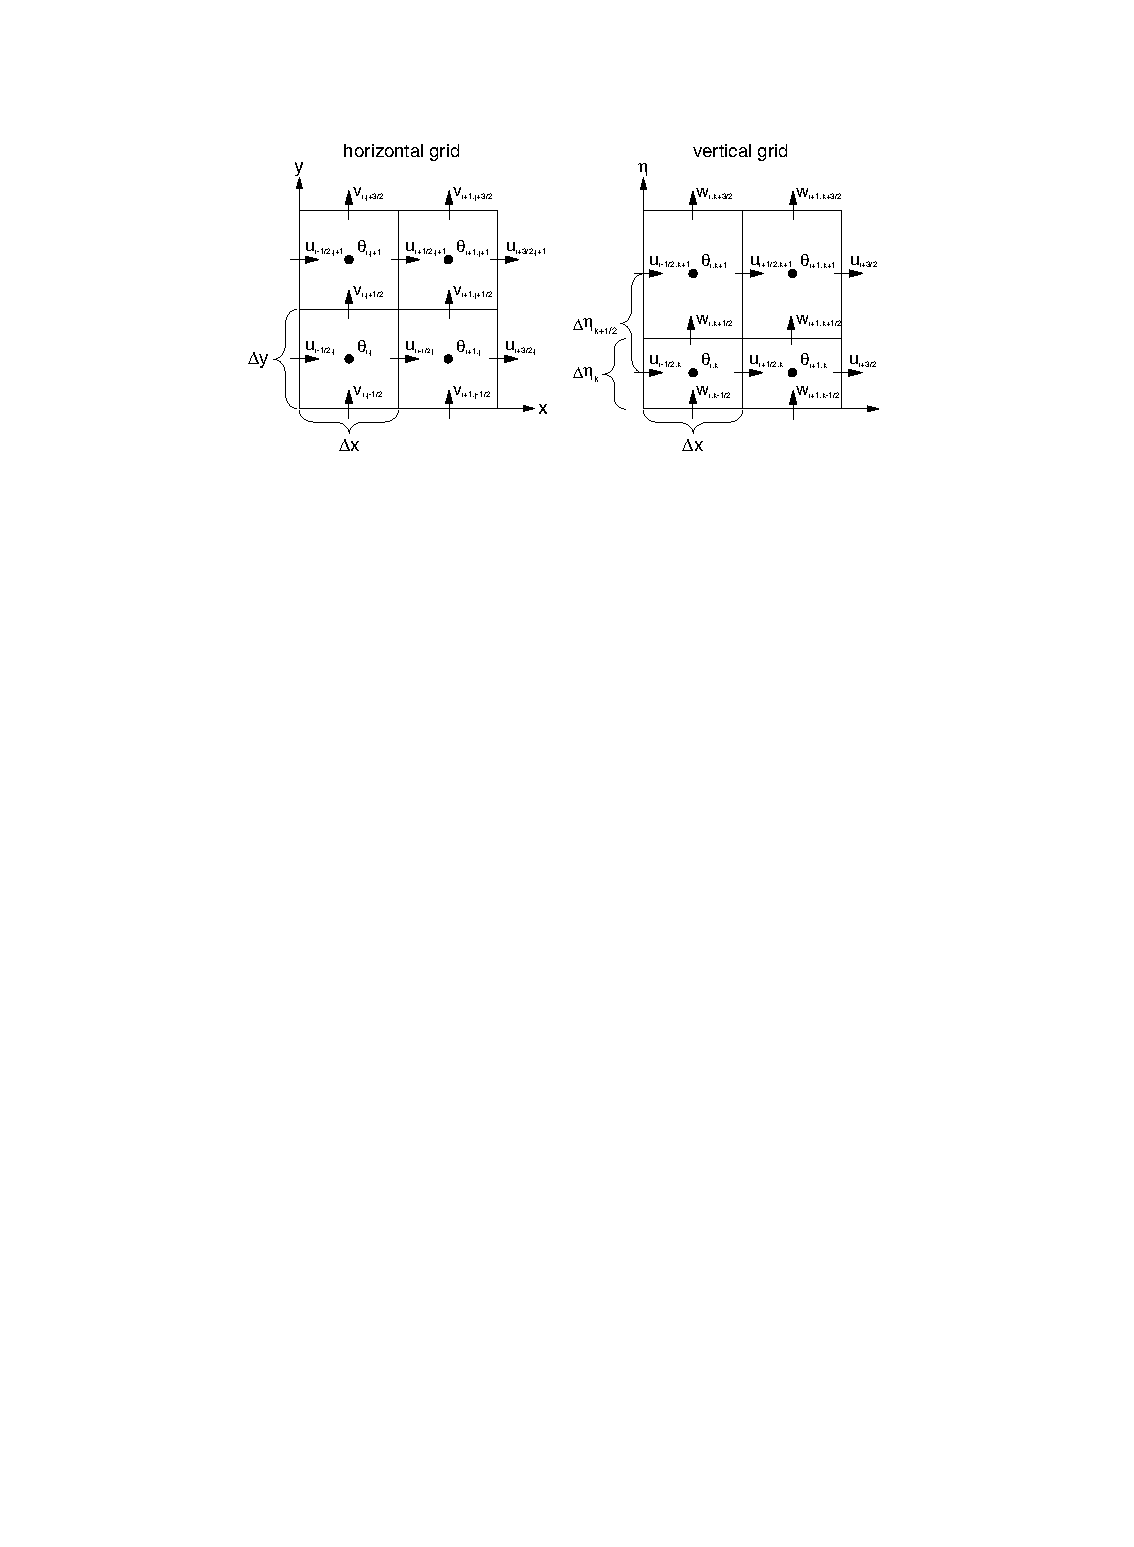
\includegraphics[width=\textwidth]{model_methods/gridstagger.pdf}
\caption{This figure is shown as presented in~\citet{Skamarock2008}, and shows the staggering of the C-grid. The horizontal staggering to the left, and the vertical staggering to the right.}
\label{fig:stagger}
\end{figure}

The time integration in ARW is performed by a "time split integration scheme", which means that the low frequency, meteorologically significant modes are integrated by a third order Runge-Kutta (RK3) integration scheme, while the higher frequency acoustic modes are integrated with a shorter time step, to conserve the numerical stability. In general, it is preferred to use as large a time step as possible while keeping the numerical stability. For integration by the RK3 scheme the maximum time step $\Delta t_{max}$ is found through equation~\ref{eqn:tmax}
\begin{equation}
\Delta t_{max} < \frac{C\cdot \Delta x}{\sqrt{3}\cdot u_{max}}
\label{eqn:tmax}
\end{equation}
where $C$ is the maximum Courant number, which depends on the order of the discretization of the advection terms. Typically in WRF, it is recommended that $\Delta t$ (in seconds) does not exceed 6 times $\Delta x$ (in km). When running the modeling system with a horizontal resolution of 4~km grid point spacing I therefore chose $\Delta t = 24$. Details about the model runs and choices of physics in the model is presented in the next section.

%---------------------
\section{Model setup}
\label{sec:modelsetup}
%---------------------
The model was ran with a 4~km$\times$4~km horizontal grid point spacing, with 300$\times$300 grid points, and 72 vertical layers, with the model top at 10~hPa.
The area covers parts of the Beaufort Sea, by Canada and Alaska. This area was chosen because data from the area has been used for related studies~\citep{Intrieri2002,Shupe2004,Kay2009,Wu2012,Palm2010,Schweiger2008} %@@@sjekk dette!!,
as mentioned in Chapter~\ref{chap:introduction}. The area is not completely ice free any part of the year~\citep{NSIDC}, and provides a good place to simulate cloud-sea ice interaction. The area is over several time zones but is approximately 7 hours behind UTC time. The times given in the WRF-ARW modeling system are UTC. The model was run for a period of 5~days, 1st to 6th of September 2012. This is approximately when the record low ice extent in the Arctic was set (eg. National Snow and Ice Data Centre, U.S.A.,~\citep{NSIDC}).

The vertical layers in the ARW model are often referred to as eta levels, because of the choice of $\eta$ as the vertical coordinate. These levels have uneven vertical spacing and the altitude of each level is dependent on pressure, therefore the level height varies in both time and space. As a consequence of pressure dependence, the levels in the lower troposphere are closer to each other than the levels higher up in the troposphere. Thus the low clouds in the area can be resolved. Approximate heights for the lowest 11 eta levels are shown in Table~\ref{tab:etaheights}.

\begin{table}[H]
\centering
\caption{Approximate height for each level in meters above the surface.}
\label{tab:etaheights} 
\begin{tabular}{C{4.cm} C{5.cm}}
\centering
\textbf{Eta level} & \textbf{Approximate height}\\ \hline
1 & 10~m\\
2 & 50~m\\
3 & 130~m\\
4 & 230~m\\
5 & 370~m\\
6 & 530~m\\
7 & 650~m\\
8 & 950~m\\
9 & 1250~m\\
10 & 1400~m\\
11 & 1600~m
\end{tabular}
\end{table}

%------------------------------------------
\subsection{Choices of physics in the model}
%------------------------------------------
The selection of physics schemes in WRF-ARW are numerous and fall into several categories, each containing several choices. Table~\ref{tab:physics} shows some of the different categories and the choice of scheme, for this study, within each of those categories.

\begin{table}[H]
\centering
\caption{Table of physics categories and choice of scheme for this thesis}
\label{tab:physics} 
\begin{tabular}{L{4cm} L{7cm}}
\centering
\textbf{Physics categories} & \textbf{Scheme selected within category}\\ \hline
(1) microphysics & aerorol-aware ~\citep{Reisner1998, Thompson2004, Thompson2008, Thompson2014}. Option 28.\\
(2) cumulus parameterization & Grell 3D  @cite authors. Option 5.\\
(3) planetary boundary layer (PBL) &  Yonsei University scheme @cite authors. Option 1.\\
(4) land-surface model & Noah Land Surface Model @cite authors. Option 2.\\
(5) radiation & RRTMG LW \& SW ~\citep{Mlawer1997, Iacono2000, Iacono2003, Iacono2008}. Radiation option 4 in both LW and SW.
\end{tabular}
\end{table}

The ARW model offers a wide selection of schemes to treat different physics that one wants represented in the model. The schemes treat the physics slightly differently and some schemes are better for certain horisontal and vertical resolutions than others, so one needs to be careful when choosing how the model is to treat the physics. For my thesis, the especially relevant scheme to mention is the cloud microphysics scheme that I chose, which is the aerosol-aware scheme described in~\citet{Thompson2014}. When studying cloud and radiation response to removal of sea ice one might expect an increase in aerosols from the open ocean and increased sea traffic. The aerosols are therefore also relevant for the choice of schemes, and the aerosol-aware scheme, described further below, includes the necessary processes for this study.

The choice of cumulus parameterization was based on the grid resolution, and the best fit for it. A horizontal grid point spacing of 4~km can be fine enough to not use cumulus parameterization~\citep{Thompson2014}, but in this thesis a parameterization that was more suitable for grid point spacings less than 10~km was chosen; the Grell 3D parameterization. According to~\citet{Wang2015} Grell 3D may be used on high resolution, like my 4~km grid point spacing.
%---------
%Yonsei University scheme was chosen for the PBL. It is a non-local-K scheme with explicit entrainment layer and parabolic profile in unstable mixed layer~\citep{Wang2015}.
%---------
%The land-surface model choice came to Noah Land Surface Model. The Noah Land Surface Model, is a unified NCEP/NCAR/AFWA (National Centers for Environmental Prediction, National Centre for Atmospheric Research, Air Force Weather Agency) scheme with soil temperature and moisture in four layers which provides sensible and latent heat fluxes to the PBL scheme~\citep{Wang2015}. Additionally, it predicts soil ice, and fractional snow cover effects, which could be important in the Arctic, but it is probably not the most important choice, since there is very little land in the area investigated, see figure~\ref{fig:area} in Chapter~\ref{chap:introduction}.
%----------
%The radiation schemes were chosen simply because they are the best match for the microphysics scheme at the time of writing. According to~\citet{Thompson2014} the Rapid Radiative Transfer Model (RRTM) for General Circulation Models (GCMs) (RRTMG) schemes for SW and LW are the only radiation schemes which include the effects of the effective radii calculated in aerosol-aware. The RRTMG schemes are accurate schemes using look-up tables for efficiency, and accounts for multiple bands and microphysics species, and includes the Monte Carlo Independent Column Approximation (MCICA) method of random cloud overlap~\citep{Wang2015}.

%------------------------------------------
\subsubsection{The aerosol-aware scheme}
%------------------------------------------
The microphysics includes explicitly resolved water vapor, cloud, and precipitation processes. The aerosol-aware scheme was chosen so that the study would have scavenging of aerosols included and have proper enough representation of aerosols to study aerosol-cloud interactions, without using the WRF model coupled with chemistry (WRF-Chem).
According to the ARW User's Guide by~\citet{Wang2015}, the aerosol-aware scheme considers water- and ice-friendly aerosols, and a climatological dataset may be used to specify initial and boundary conditions for the aerosol variables. I have used this climatological dataset, which will be explained in Subsection~\ref{subsec:inputdata}~Input~data. The scheme uses a monthly mean for aerosol number concentrations derived from multi-year (2001-2007) global model simulations in which particles and their precursors are emitted by natural and anthropogenic sources and are explicitly modeled with multiple size bins for multiple species of aerosols by the Goddard Chemistry Aerosol Radiation and Transport (GOCART) model %(@desiterteGinoux2001)
~\citep{Thompson2014}.
The aerosol-aware scheme~\citep{Thompson2014} is built on the schematic shown in figure~\ref{fig:microphysics}, from~\citet{Reisner1998}. It is a double moment scheme, which means it computes both mass mixing ratios, Q, and number concentrations, N, for the same water species (hydrometeors). 

\begin{figure}[h]
\centering
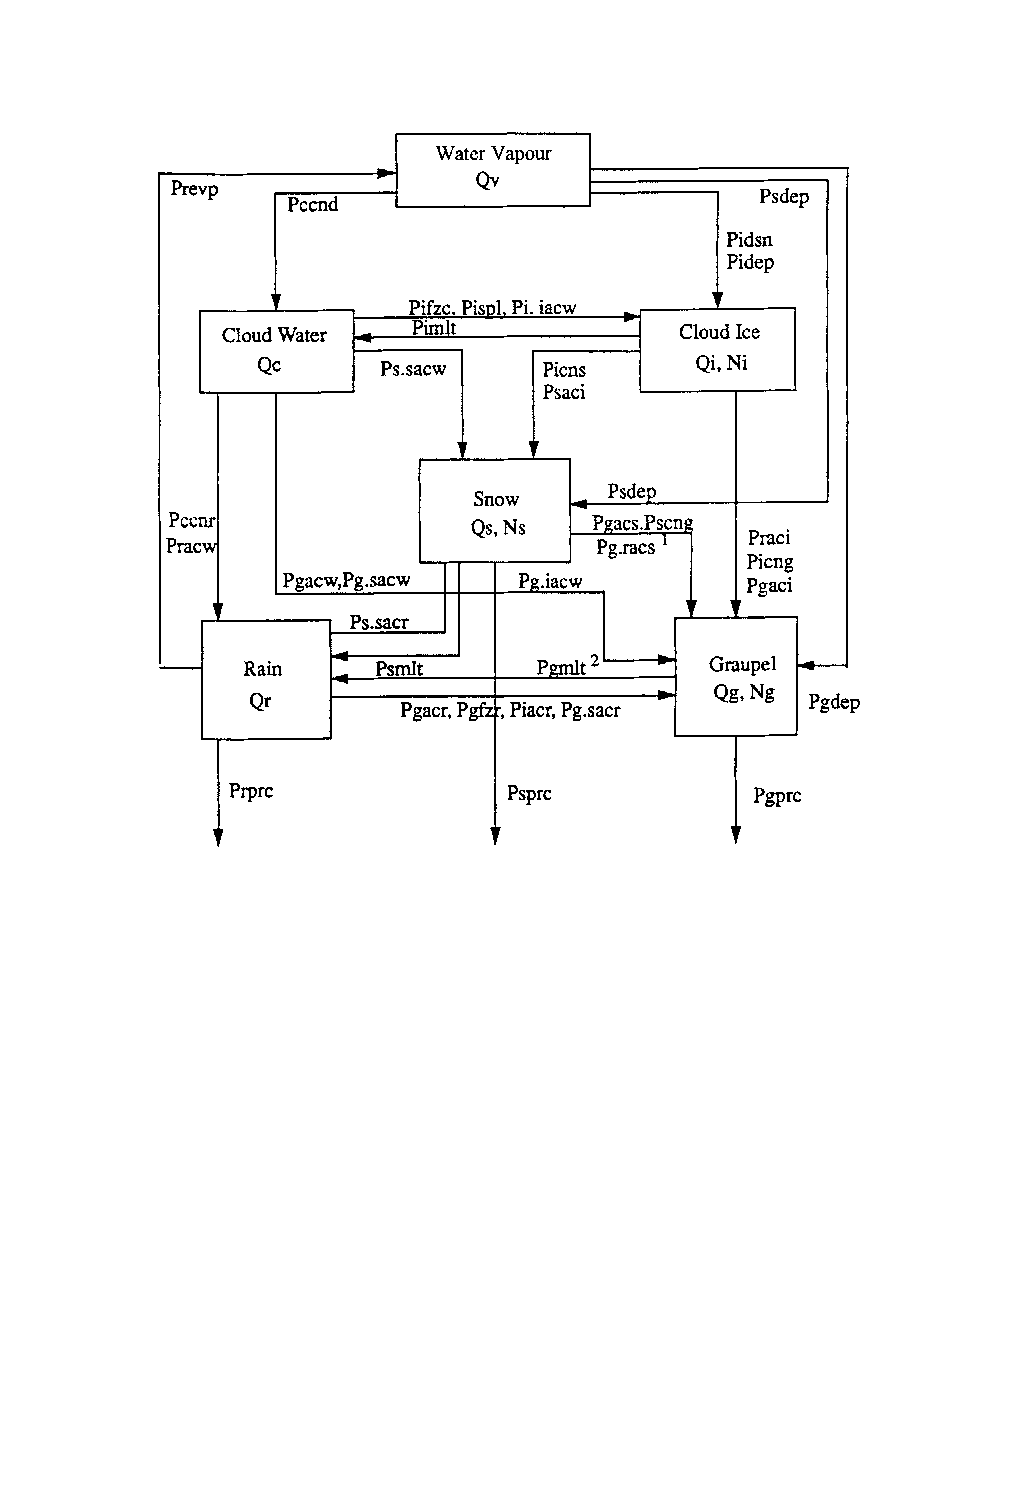
\includegraphics[width=0.9\textwidth]{model_methods/microphysics.pdf}
\caption{Cloud microphysical parameterization scheme used in some NWP models as shown in~\citet{Reisner1998}. A full list of the acronyms used in the schematic can be found in~\citet{Reisner1998}.}
\label{fig:microphysics}
\end{figure}

Figure~\ref{fig:microphysics} show the processes in the microphysics scheme developed by~\citet{Reisner1998}, which the first bulk microphysics scheme by Thompson~\citep{Thompson2004} was based on. The aerosol-aware scheme~\citep{Thompson2014} is an extension of the updated Thompson bulk microphysics scheme described in~\citet{Thompson2008}. The figure shows a schematic of five hydrometeors, cloud water (c), rain (r), ice (i), snow (s) and graupel (g), and if just the mass mixing ratio is calculated or if both the mass mixing ratio and the number concentration is calculated. For each of the hydrometeors, prognostic equations are used with all the sources and sink terms included.
 % which was originally built on this~\citep{Thompson2004}, but there is not much left of it in the code now (@cite the code comments?).
 
%------------------------------------------
\subsubsection{The RRTMG radiation schemes}
%------------------------------------------
According to~\citet{Thompson2014} the Rapid Radiative Transfer Model (RRTM) for General Circulation Models (GCMs) (RRTMG) schemes for SW and LW~\citep{Mlawer1997, Iacono2000, Iacono2003, Iacono2008} are the only radiation schemes which include the effects of the effective radii calculated in aerosol-aware. These were therefore used in combination with the aerosol-aware cloud microphysics scheme. The RRTMG schemes are accurate schemes using look-up tables for efficiency, and accounts for multiple bands and microphysics species, and includes the Monte Carlo Independent Column Approximation (MCICA) method of random cloud overlap~\citep{Wang2015}.
%The RRTM scheme described in~\citet{Mlawer1997} uses the correlated-k method, which is an approximated technique for the accelerated calculation of fluxes and cooling rates for inhomogeneous atmospheres~\citep{Mlawer1997}. %\textbf{@define inhomogeneous atmosphere}.
%The correlated-k method is capable of achieving accuracy comparable with that of line-by-line models with an extreme reduction in the number of radiative transfer operations performed~\citep{Mlawer1997}, which by that reduces computational cost and increases computational efficiency. The Line-By-Line Radiative Transfer Model (LBLRTM) is used both to calculate the absorption coefficients used to generate the k distributions needed by RRTM and  to evaluate the RRTM calculations of fluxes and cooling rates~\citep{Iacono2000}. 

%---------------------
\section{Model runs}
%---------------------
The results presented in the next chapter are based on four different runs. The control run is the run where the aerosol climatological dataset has been used unchanged, and where the sea ice is kept as it was in the downloaded input data, see Subsection~\ref{subsec:inputdata}. The control run is used as a base to compare the other runs to, those with no ice and/or increased aerosol number concentrations.

There are two runs where the sea ice was removed, NoIce and Aero10NoIce. The point of this is to compare the run with no ice to the control run, and see if there are any changes in the cloud properties, and SW and LW fluxes. For one of those runs the aerosol number concentration was also increased, results from this run can be compared with the control run.

The number of water- and ice-friendly aerosols were multiplied by 10 both with and without sea ice for two runs: Aero10 with ice, and as mentioned above, Aero10NoIce without ice. The goal is to find changes in cloud properties, and radiation fluxes compared to those in the control run.

Table~\ref{tab:runs} shows an overview of the different runs that have been executed, whose output have been used for production of figures presented in the next chapter.

\begin{table}[H]
\centering
\caption{Table showing the names of the runs and if they have sea ice or not, and if the aerosol concentration has been increased by a factor of 10 through input files. All the runs have the same horizontal resolution of 4~km$\times$4~km, dimensions 300$\times$300, 72 vertical layers and $\Delta t$=24~s.}
\label{tab:runs} 
\begin{tabular}{L{2.3cm} L{2cm} L{3cm}}
\centering
Name & Sea ice & Aerosol concentration\\ \hline
control & initial & climatology\\
NoIce & removed & climatology\\
Aero10 & initial & climatology$\times$10\\
Aero10NoIce & removed & climatology$\times$10\\
\end{tabular}
\end{table}

%---------------------
\subsection{Input data}
\label{subsec:inputdata}
%---------------------
The model runs were initialized with data downloaded from the European Centre for Medium-Range Weather Forecasts (ECMWF). %~\citet{ecmwf}
%@cite web page.%was downloaded from their site and used as input for initial and boundary?? conditions.
The downloaded data is from the ERA-Interim data set, which is a global atmospheric reanalysis from 1979 to present and continues to be updated in real time. %~\citet{ecmwf}.%@make bib for ecmwf
Through WPS the data from ERA-Interim was interpolated over the area, with a 2 degree minute spacing between the points, to be used to initialize the model. The data used is in 6-hourly atmospheric fields on pressure levels, for the first five days of September 2012, which was the period the model was run for. This is done to make sure the initial meteorological conditions are the same in every run, so that the effects of changing a variable in the input files for the modeling system are only due to that change.

To use the climatological aerosol data set, the file containing monthly means had to be called through WPS. The aerosol input data includes mass mixing ratios of sulfates, sea salts, organic carbon, dust, and black carbon from a 7-yr simulation with 0.5$\degree$ longitude by 1.25$\degree$ latitude spacing~\citep{Thompson2014}.

\subsection{Manipulation of input files}
The input files for the ARW solver, created by WPS and REAL (see figure~\ref{fig:wrfflowchart}) were manipulated by use of the NetCDF Operator (NCO) tool ncap2. In these files the sea ice was removed for the runs without sea ice (NoIce and Aero10NoIce) and the aerosol number concentration from the climatological dataset was multiplied by 10 for the runs with increased aerosol number concentration (Aero10 and Aero10NoIce).

%---------------------
\section{Processing the model output}
%---------------------
Figures presented in my thesis, I made (unless other is stated) by use of NCL (National Center for Atmospheric Research (NCAR) Command Language). For the NCL scripts I found a lot of help and inspiration from the example scripts for WRF-users.% available at @(URL for examples).

The model output was stored as instantaneous values for every hour for each of the five days, from each of the four runs. 

To study the response in cloud radiative properties, all fields of interest were made into daily time averages, by use of NCL, in each run. Some fields vary only in horizontal space and in time (2-dimensional in space), and were simply added together and divided by the number of hours in that day. These fields are: SW and LW radiation down at the surface and up at TOA, latent heat (LH) and sensible heat (SH), temperature at the surface and at 2~m height and winds at 10~m height.

The cloud parameters, such as $r_e$ and CDNC, vary also in the vertical (3-dimensional in space) and have been averaged over the 11 lowermost layers (the lower $\sim$1600~m above the surface) and all hours of the day. Hence, the figures showing $r_e$ and CDNC over maps do not account for variations in the vertical.

The LWC on the other hand has not been averaged over the layers, but summarized into LWP. In each of the lowermost 11 layers the LWC has been multiplied with the thickness of the respective layer and then added in height to make the LWP.

The differences between two runs, presented in the next chapter, are daily time averaged differences. Where the difference has been calculated for every hour of the day, and then averaged in time.